\begin{frame}{Fog/Cloudlet/Swarmbox \& New Infrastructure}
  \begin{columns}
    \column{0.5\textwidth}
    \begin{figure}
      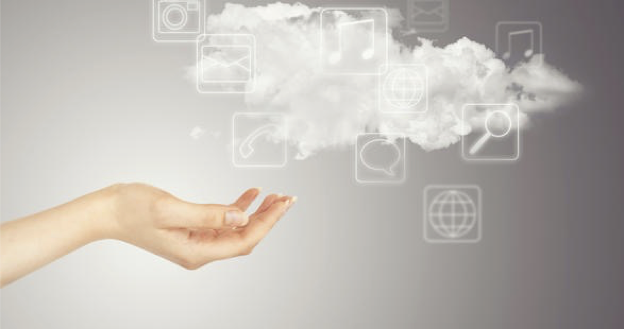
\includegraphics[width=0.8\textwidth]{figures/fog.png}
      \captionsetup{labelformat=empty}
      \caption{Cisco Fog Computing~\cite{bonomi2012fog}}
    \end{figure}
    \pause
    \column{0.5\textwidth}
    \begin{figure}
      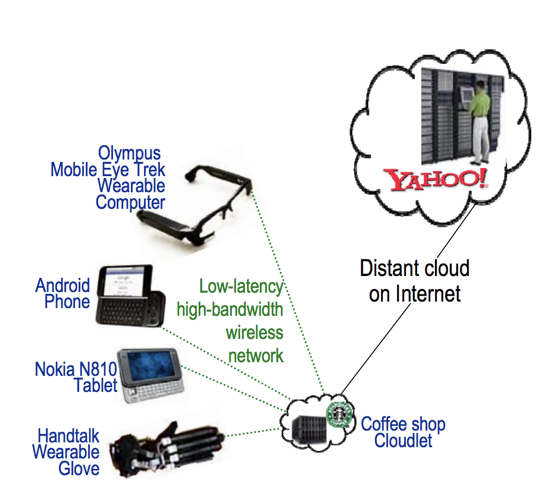
\includegraphics[width=0.8\textwidth]{figures/cloudlet.png}
      \captionsetup{labelformat=empty}
      \caption{Cloudlet~\cite{satyanarayanan2009case}}
    \end{figure}
  \end{columns}
  \pause
  \begin{figure}
    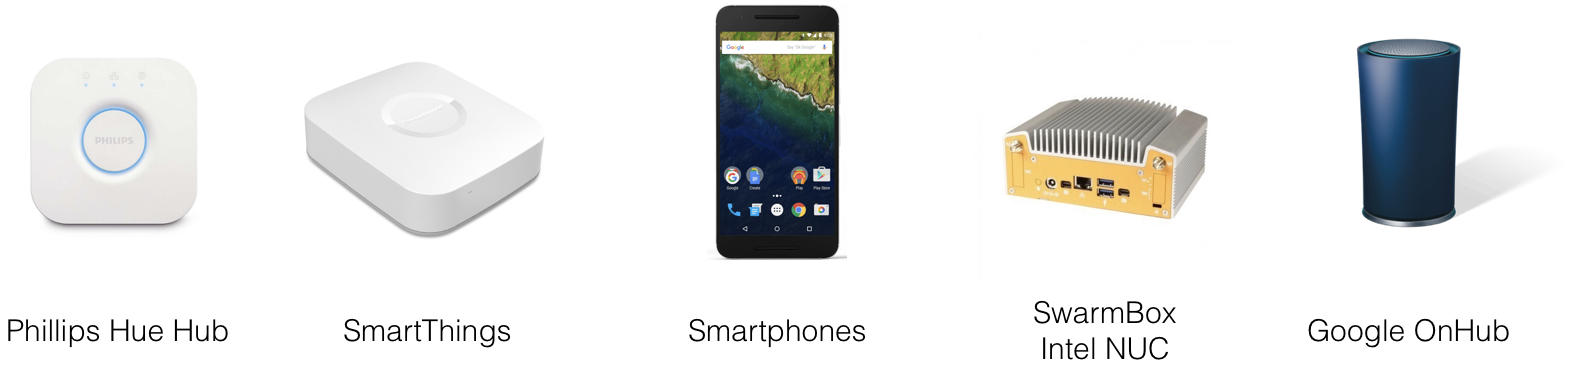
\includegraphics[width=0.8\textwidth]{figures/gateways.png}
    \captionsetup{labelformat=empty}
    \caption{Many Gateways}
  \end{figure}
\end{frame}

\begin{frame}{Heterogeneous Environment}
  \vspace{1em}
  \begin{figure}
    \centering
    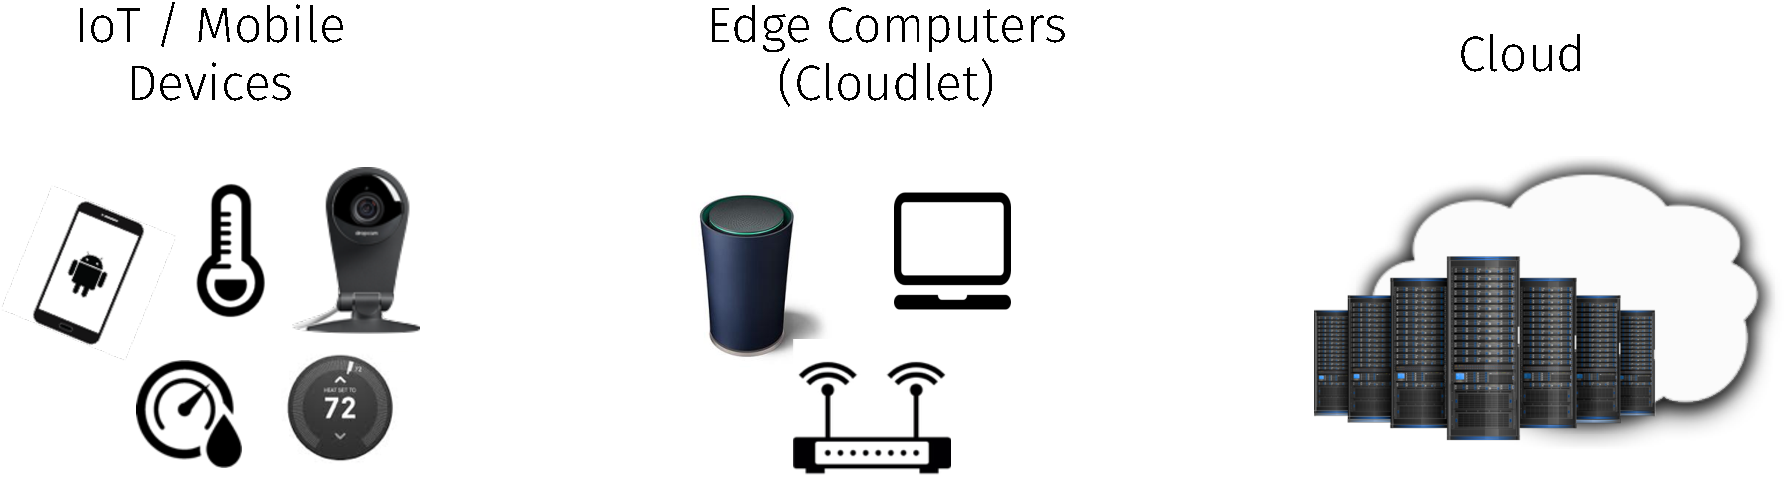
\includegraphics[width=0.95\linewidth]{figures/heterogeneous-1.pdf} \\
    \vspace{1em}
    \only<1>{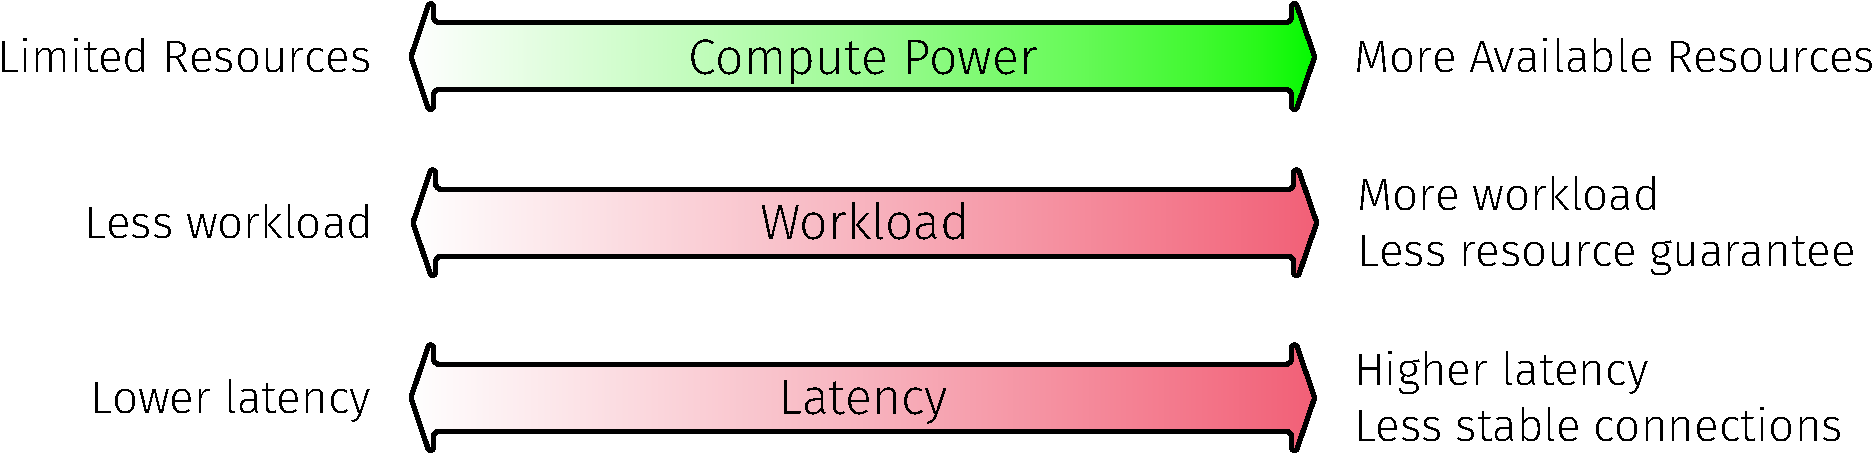
\includegraphics[width=0.95\linewidth]{figures/heterogeneous-2.pdf}}
    \vspace{1em}
    \only<1>{\caption{Characteristics of IoT/mobile, edge and cloud}}
  \end{figure}

  \only<2>{
    \begin{columns}
      \column{0.4\textwidth}
      \begin{figure}
        \centering
        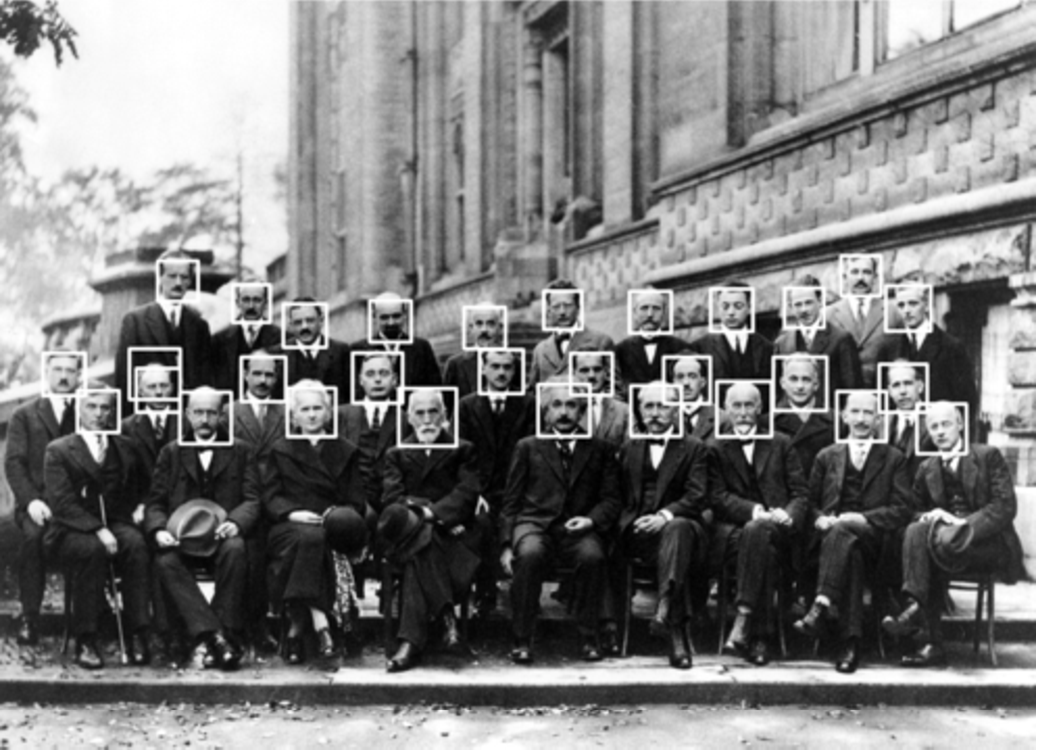
\includegraphics[width=\textwidth]{figures/physicist.pdf}
      \end{figure}
      
      \column{0.6\textwidth}
      \begin{table}
        \footnotesize
        \centering
        \begin{tabular}{c c c}
          \toprule
          \specialcell{RPi\\Model B}
          & \specialcell{Macbook \\ Model A1502}
          & \specialcell{Workstation\\(Xeon E5-1620)} \\
          \midrule
          4105 & 544 & 346 \\
          \bottomrule
        \end{tabular}
        \caption{Processing times (ms) on different platforms.}
      \end{table}
    \end{columns}
  }
\end{frame}

\begin{frame}{Accuracy and Processing Times Tradeoff}
  \metroset{block=fill}
  \begin{columns}
    \column{0.5\textwidth}
    \begin{block}{Adaptation}
      Within the accuracy and processing times tradeoff space, select
      appropriate algorithm and parameters to meet bounded response time goal.
    \end{block}
    \column{0.5\textwidth}
    \begin{tikzpicture}
      \begin{axis}[
        width  = \textwidth,
        xlabel = Processing Times (normalize),
        ylabel = Accuracy,
        ymin   = 0,
        ymax   = 1,
        ytick  = {0, 1},
        xmin   = 0,
        xmax   = 1,
        xtick  = {0, 1},
        ]

        \draw [densely dotted] (axis cs: 0.55, 0.69) -- (axis cs: 0.55, 0);
        \draw [densely dotted] (axis cs: 0.55, 0.69) -- (axis cs: 0, 0.69);

        \addplot[color=red, mark=x, only marks] coordinates {(0.55, 0.69)};
        \addplot[color=blue, mark=x, only marks] coordinates {(0.95,0.95)};
        \addplot[color=blue, mark=x, only marks] coordinates {(0.90,0.92)};
        \addplot[color=blue, mark=x, only marks] coordinates {(0.85,0.90)};
        \addplot[color=blue, mark=x, only marks] coordinates {(0.70,0.80)};
        \addplot[color=blue, mark=x, only marks] coordinates {(0.75,0.75)};
        \addplot[color=blue, mark=x, only marks] coordinates {
          (0.6, 0.7)
          (0.5, 0.65)
          (0.4, 0.55)
          (0.3, 0.50)
          (0.2, 0.45)
          (0.1, 0.20)
        };
        \addplot[color=blue, mark=x, only marks] coordinates {
          (0.83, 0.62)
          (0.80, 0.59)
          (0.74, 0.60)
          (0.63, 0.56)
          (0.61, 0.36)
          (0.51, 0.34)
          (0.50, 0.40)
          (0.49, 0.41)
          (0.47, 0.42)
          (0.46, 0.30)
          (0.44, 0.25)
          (0.24, 0.20)
          (0.10, 0.10)
        };
      \end{axis}
    \end{tikzpicture}
  \end{columns}
\end{frame}

\begin{frame}{Accuracy and Processing Times Tradeoff}
  \begin{figure}
    \begin{subfigure}[t]{0.45\textwidth}
      \centering
      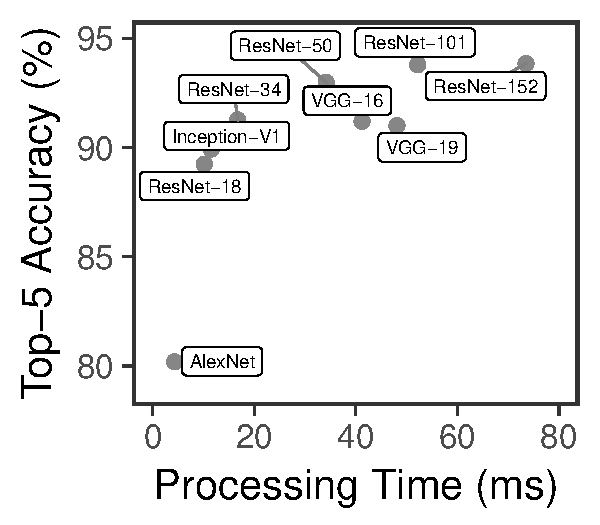
\includegraphics[width=0.95\linewidth]{figures/motiv-functions.pdf}
      \caption{Benchmarks for popular convolutional neural network (CNN)
        models. Data source: \url{https://github.com/jcjohnson/cnn-benchmarks}.}
    \end{subfigure}
    \hfill
    \begin{subfigure}[t]{0.45\textwidth}
      \centering
      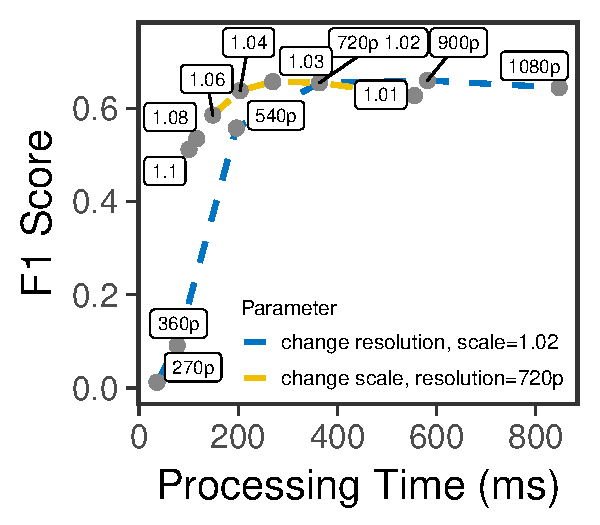
\includegraphics[width=0.95\linewidth]{figures/motiv-params.pdf}
      \caption{Benchmarks for Viola Jones face detection when changing different
        parameters (see explanation on the next slide).}
    \end{subfigure}
  \end{figure}
\end{frame}

%%% Local Variables:
%%% mode: latex
%%% TeX-master: "../talk"
%%% TeX-engine: xetex
%%% End:
